\documentclass{article}
\usepackage{graphicx}
\usepackage{hyperref}
\usepackage[utf8]{inputenc}

\graphicspath{ {./images/} }

\title{Simulazione della trasmissione simultanea di quattro segnali su un'unica linea utilizzando la tecnica FDM}
\author{Lena Giovanni Leonardo}
\date{Marzo 2022}

\begin{document}

\maketitle

\section{Scopo del progetto}
Lo scopo del progetto è la realizzazione di una simulazione software per la trasmissione di quattro segnali (due digitali
e due analogici) mediante lo stesso mezzo utilizzando la tecnica del frequency-division multiplexing (o FDM) \cite{fdm}.\\
I quattro segnali hanno la stessa frequenza e prima di essere trasmessi vengono modulati, ciascuno con una frequenza
portante diversa in modo da non avere sovrapposizioni di banda. Inoltre, tra un segnale e l'altro è prevista una
banda di guardia per evitare ulteriormente le interferenze tra un segnale e l'altro.\\
Ad ogni stadio è inoltre possibile visualizzare interattivamente ed in tempo reale i segnali, in modo da poterne comprendere
meglio il funzionamento. Viene inoltre mostrato lo spettro del segnale multiplexato, ottenuto applicando un algoritmo di
Fast Fourier Transform (FFT) \cite{fft} ed è possibile introdurre un segnale di disturbo per osservare gli effetti sui segnali demodulati
finali.\\
È infine presente un controllo che permette di rallentare il tempo per osservare meglio la generazione, modulazione e demodulazione
dei segnali. Per questioni di performance, la simulazione inizia con l'andamento del tempo rallentato di 10 volte.

\section{Strumenti utilizzati}
La simulazione è interamente programmata nel linguaggio di programmazione Rust \cite{rust}, principalmente per le velocità che
permette di raggiungere e che non sono comparabili a nessun linguaggio di scripting interpretato come Python. La libreria
per l'interfaccia grafica si chiama egui \cite{egui}, tutti gli algoritmi per la generazione delle onde e per il filtro sono stati
implementati con gli strumenti matematici che offre il linguaggio, fatta eccezione per l'algoritmo di Fast Fourier Transform,
utilizzato per fini grafici, che viene dalla libreria rustfft \cite{rustfft}.

\section{Cenni teorici}
\subsection{Frequency-division multiplexing}
La tecnica della multiplazione a divisione di frequenza (in breve FDM) consiste nella suddivisione della banda totale disponibile
in una serie di bande più piccole e non sovrapposte tra loro, nelle quali ogni segnale può essere trasmesso indipendentemente
dagli altri e allo stesso tempo.\\
Questa tecnica si differenzia da altre tecniche come TDM che invece si basano sulla divisione del tempo, assegnando quindi
ad ogni segnale una finestra temporale ed alternando continuamente tra di esse.\\
Esempi comuni di FDM si trovano all'interno della trasmissione televisiva e radiofonica, in cui frequenze diverse vengono
trasmesse tutte allo stesso tempo. La selezione del canale, infatti, avviene sintonizzandosi su una specifica frequenza.
Ciò consente la trasmissione di una grossa quantità di dati simultaneamente, senza sprechi di banda.

\section{I segnali generati}
La frequenza di campionamento della simulazione è di $2.5 MHz$, che corrisponde ad un periodo di $400 ns$. Secondo il teorema
del campionamento di Nyquist-Shannon, è sufficiente che la frequenza di campionamento sia il doppio della frequenza massima
che si intende campionare.\\
All'interno della simulazione, si raggiungono frequenze ben inferiori alla metà della frequenza di campionamento, tuttavia
per essere sicuri del corretto funzionamento, è stata scelta una frequenza superiore. Dato il periodo molto ristretto ($400 ns$),
non è computazionalmente possibile eseguire l'algoritmo in tempo reale. Oltre alla generazione dei segnali, infatti, ogni
sample viene sottoposto a vari algoritmi per la visualizzazione, modulazione e demodulazione che verranno approfonditi
successivamente.

\begin{itemize}
    \item Onda sinusoidale a 20 kHz
    \item Onda quadra a 20 kHz
    \item Onda a dente di sega a 20 kHz
    \item Onda quadra contenente un messaggio di testo a 20 kHz
\end{itemize}

\section{Modulazione dei segnali}
Prima di poter essere trasmessi, i segnali devono essere modulati ad una frequenza superiore. Dato che si sta utilizzando la
tecnica FDM per la trasmissione dei segnali, è molto importante che le modulazioni avvengano ognuna ad una frequenza differente
dall'altra. È fondamentale calcolare la banda dei segnali modulati e fare in modo che un segnale non si sovrapponga con l'altro.
Per garantire una maggiore sicurezza viene inoltre considerata una banda di guardia nella quale non è presente alcun segnale.\\
In alcune modulazioni (ad esempio FM), la banda teorica risultante è infinita. Secondo la regola di Carson, la banda utile nella
quale ricadono il 98\% delle frequenze è comunque limitata, tuttavia per una modulazione migliore è possibile applicare un filtro
passa banda al segnale prima che esso venga unito agli altri per la trasmissione su un unico mezzo.\\

Le modulazioni progettate per i segnali trasmessi sono riportate di seguito:

\subsection{1. Onda sinusoidale modulata in FM}
\begin{equation}
    f_m = 20 kHz
\end{equation}

\begin{equation}
    \Delta f = 75 \hspace{0.1cm} kHz
\end{equation}

\begin{equation}
    B = 2 \cdot (f_m + \Delta f) = 190 kHz
\end{equation}

\subsection{2. Onda quadra modulata in FSK}
\begin{equation}
    f_m = 20 kHz
\end{equation}

\begin{equation}
    \Delta f = 75 \hspace{0.1cm} kHz
\end{equation}

\begin{equation}
    B = 2 \cdot (\Delta f + f_m) = 190 kHz
\end{equation}

\subsection{3. Onda a dente di sega modulata in AM}
\begin{equation}
    f_m = 20 kHz
\end{equation}

\begin{equation}
    B = 2 \cdot f_m = 40 kHz
\end{equation}

\subsection{4. Onda quadra modulata in OOK}
\begin{equation}
    f_m = 20 kHz
\end{equation}

\begin{equation}
    B = 6 \cdot f_m = 120 kHz
\end{equation}

\begin{center}
    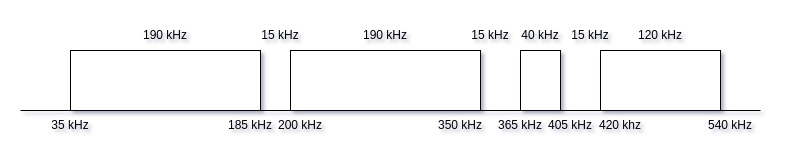
\includegraphics[width=\textwidth]{bandwidth.png}
\end{center}
Lo spettro finale, ottenuto dal calcolo delle bande e lasciando 15 kHz come bande di guardia.

\section{Unione dei segnali con un multiplexer FDM}
Una volta che i segnali sono stati generati e modulati con delle portanti adeguatamente dimensionate, la trasmissione in FDM
avviene semplicemente sommando i quattro segnali. È possibile verificare l'efficacia di questa tecnica attraverso il grafico
dello spettro del segnale. Nel caso di corretta modulazione dei segnali, dovrebbe essere possibile visualizzare quattro gruppi
di frequenze, ognuna separata dall'altra da un vuoto più o meno grande, che rappresenta le frequenze di guardia.

\section{Separazione di ogni singolo segnale}
Per poter demodulare ed ottenere i segnali originali, è necessario isolare la banda di frequenze utili attraverso un filtro
passa-banda opportunamente dimensionato.

\section{Demodulazione dei segnali}

\subsection{Demodulazione FM}
\subsection{Demodulazione FSK}
Un segnale digitale modulato in FSK è composto da un'armonica con una delle due frequenze, dette frequenze di manipolazione
($f_1$ e $f_2$) che si discostano di un fattore $\pm \Delta f$ dalla frequenza portante $f_p$ e si alternano, in base al bit
trasmesso. Ci sono vari modi per demodulare un segnale FSK all'interno di un DSP.\\
Il modo più banale è l'applicazione della trasformata di Fourier al segnale modulato, per rilevare quale delle due frequenze
di manipolazione viene trasmessa, tuttavia questo metodo è molto inefficiente (anche con le modrne implementazioni FFT) in quanto
la trasformata di Fourier rileva tutte le frequenze dello spettro, nonostante ai fini della demodulazione siano sufficienti
solo $f_1$ ed $f_2$.\\
Una tecnica molto più efficiente consiste nell'applicazione dell'algoritmo di Goertzel al segnale, che permette di rilevare
l'intensità di una singola frequenza. Applicando l'algoritmo due volte, una per $f_1$ e l'altra per $f_2$ e confrontando le due
intensità per determinare la maggiore, è semplice stabilire quale dei due bit sta essendo trasmesso ad ogni istante.

\subsection{Demodulazione AM}




\section{Sviluppi futuri}



\begin{thebibliography}{9}
    \bibitem{egui}
    \href{https://github.com/emilk/egui}{egui: an easy-to-use immediate mode GUI in Rust that runs on both web and native}

    \bibitem{fdm}
    \href{https://en.wikipedia.org/wiki/Frequency-division_multiplexing}{Frequency-division multiplexing}

    \bibitem{fft}
    \href{https://en.wikipedia.org/wiki/Fast_Fourier_transform}{Fast Fourier Transform}

    \bibitem{rust}
    \href{https://rust-lang.org}{Rust}

    \bibitem{rustfft}
    \href{https://docs.rs/rustfft/latest/rustfft/}{RustFFT is a high-performance FFT library written in pure Rust.}
\end{thebibliography}


\end{document}
